\chapter{Architecture Implementation}
In the following chapter we comment on the implementation of the individual decompositions as described in figure \ref{fig:comp}.
Current source code can be found on the project \gls{github} presented in section \ref{sec:archvcs} and a frozen state is attached to this thesis on compact disk.

It should be noted that although Astah claimed \gls{rte} support for C++, it was found to be unreliable due to poor support of the C++ namespace feature.
The application was thus developed using a conventional model-driven design approach.

Code in this project is formatted in compliance to the WebKit formatting rules presented in section \ref{sec:resformat} automatically on file save using QtCreator integration of clang-format. 

\section{Main Application}
The core functionality of the program was established in section \ref{sec:archplug} to be
\begin{itemize}
	\item Configuration storage
	\item Plugin management
	\item Curve rendering to screen
	\item \gls{cli} parsing
\end{itemize}

These components lead to a further decomposition shown in figure \ref{fig:main}.

\begin{figure}[htb]
	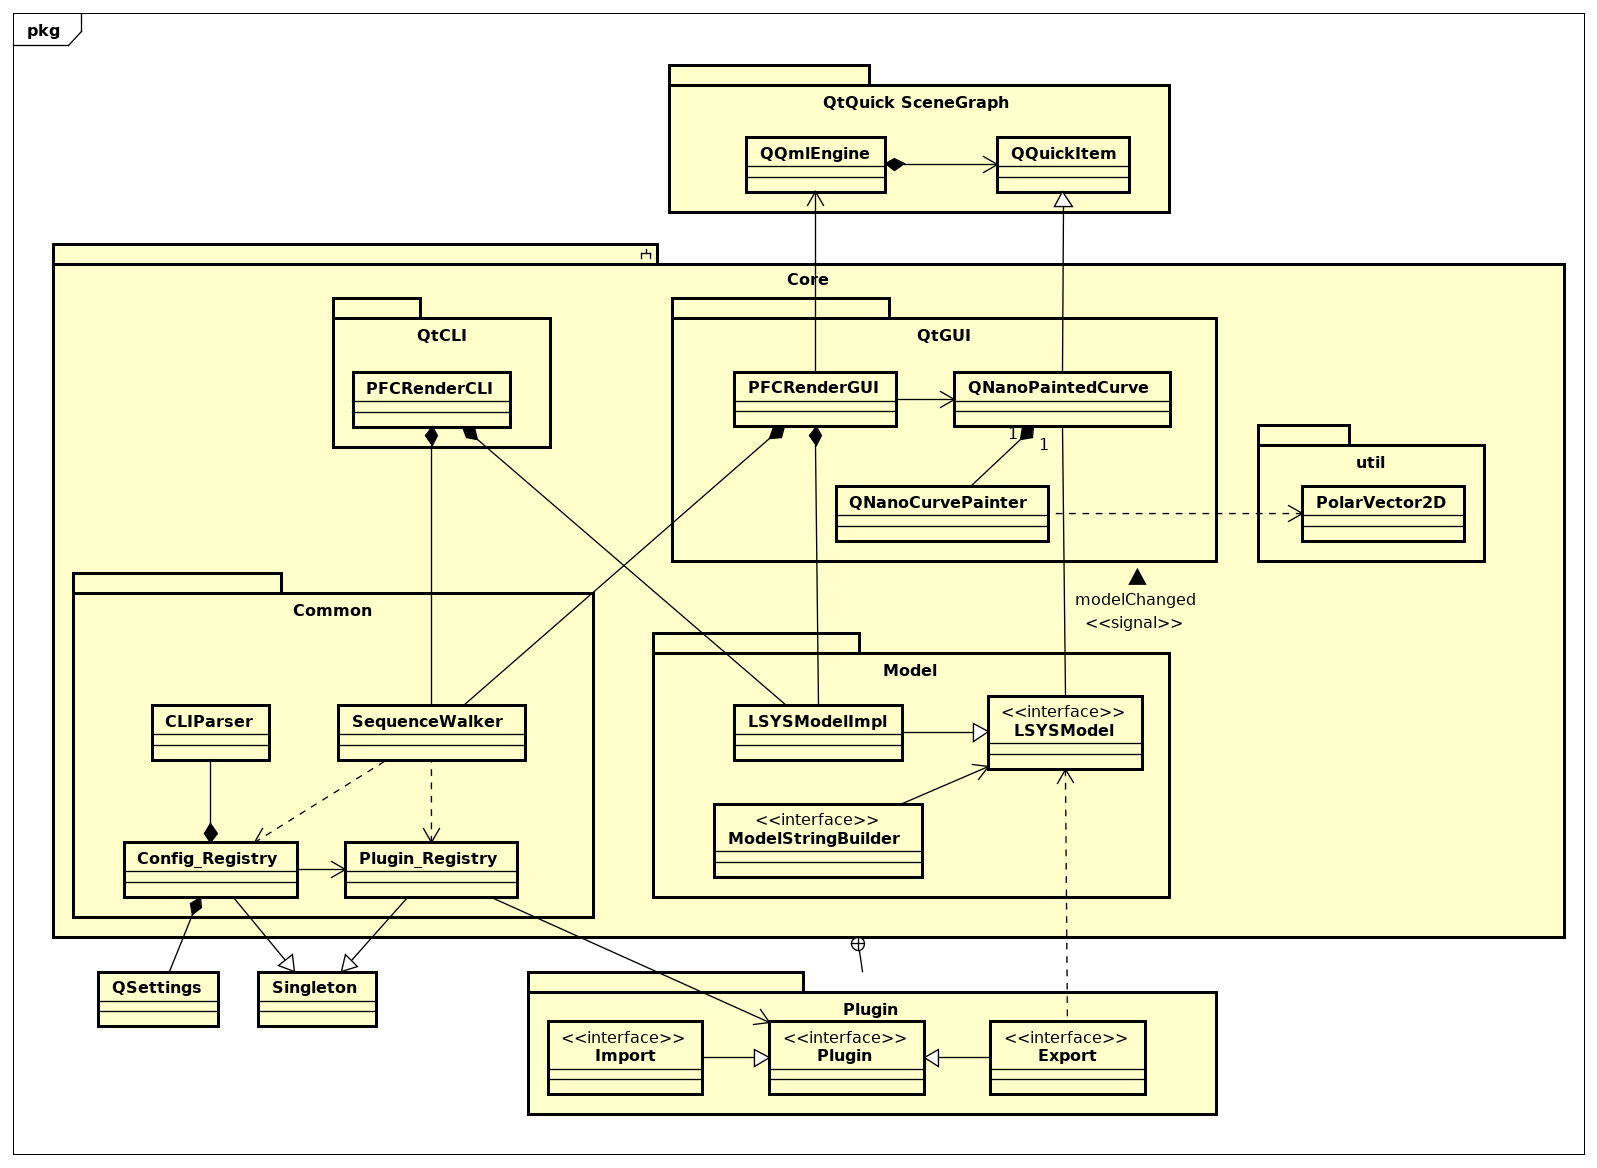
\includegraphics[width=\textwidth]{MainAppClassDiagram}
	\caption{Class Structure of Core Application}
	\label{fig:main}
\end{figure} 

\paragraph{Initialization and Operation}
The main entry point into the application is not shown in the static class diagram, but it involves creating a Qt \class{QGuiApplication} object and a \class{PFCRenderGUI} or \class{PFCRenderCLI} object.

In case of \gls{gui} operation, a \class{QQmlEngine} is instantiated to handle the declarative \gls{gui} part and the Qt event loop is executed through the \class{QGuiApplication}. Requested operations like \gls{lsys} import or PDF export are handled by a \class{SequenceWalker}, upon completion of which the \gls{gui} starts handling all further interaction asynchronously through a \gls{mos} based messaging system called \textit{Signals and Slots}.

In batch mode, the \class{PFCRenderCLI} simply calls the \class{SequenceWalker} which handles requested operations and then exits the program.

\paragraph{Configuration}
\class{Config\_Registry} is the central store of configuration information as outlined in section \ref{sec:archconf} and - upon creation of its instance, which happens the first time some class wants to access configuration data - resolves the sequence of reading settings from file, creating the \class{Plugin\_Registry} to query for options, and parsing the \gls{cli}. It is also available to the \gls{qml} part of the application as an exported \term{QML Type}, allowing \gls{gui} screens written in \gls{qml} to access config data.

\paragraph{Plugins} Since Plugins need to be loaded to query for config information anyway, it makes sense to hold references to them active, so they do not have to be loaded a second time once accessed for execution. \class{Plugin\_Registry} is a second Singleton tasked with resolving all available plugins and holds this reference associated with plugin name for simple lookup.

\paragraph{Model Creation} The model is created once on startup of the application via the \class{PFCRender*} objects. Once the sequence walker executes an import plugin, it is given a \class{ModelStringBuilder} object to execute. Upon completion, it pushes an owning \code{std::unique\_ptr<>} to that string to the model to avoid potentially costly string copying.

Benefit of returning a builder object instead of direct plugin invocation is supporting deferred / delegated execution, as it becomes simple for the sequence walker to hand the builder over to a thread. This keeps the \gls{gui} responsive while computation occurs in the background. This feature is planned for a subsequent release, as it was not a direct requirement.

\paragraph{GUI Creation} The \gls{gui} is loaded from \gls{qml} files on startup, the \class{QNanoPaintedCurve} displaying an empty rendering. It is connected to the \code{modelChanged} signal and - on notification of a change - copies the model string to its renderer - \class{QNanoCurvePainter}. It then notifies the \term{scene graph} it needs to be redrawn. When the rendering thread gets to the \class{QNanoCurvePainter} node upon re-rendering the scene graph, it invokes the \code{QNanoCurvePainter::paint()} function which parses the string into actual geometry. On completed rendering, the QNanoPaintedCurve notifies the \gls{qml} part of the \gls{gui} if its \gls{bounding box} has changed, in order to scale the result to the available window size.

\paragraph{Export} The \class{SequenceWalker} hands the model string over to the plugin, which is then free to do its job, fetching configuration from the \class{Config\_Registry}.

\subsection{Challenges Faced in Rendering the Model Curve}
Had performance not been a direct requirement, the QPainter API would have been sufficiently sophisticated to enable curve drawing. Since QPainter is too slow - as found in section \ref{sec:qtrender} - an alternative approach is necessary.

The first studied alternative was direct insertion of geometry into a \class{QSSGeometryNode} scene graph node, which turned out to be too inflexible to satisfy all requirements.

An alternative was ultimately adopted with of using QNanoPainter.

We will now discuss challenges faced with both rendering methods.

\subsubsection{QSGGeometryNode - Direct Geometry Insertion into the Scene Graph}\label{sec:impldirect}

First approach was direct creation of a \cmd{QSGGeometryNode}, which is a Qt SceneGraph frontend for direct specification of graphical primitives (\term{vertices} and \term{material}), providing a low-level abstraction on top of the rendering backends.
The code used in this approach is available on the \cmd{rendermethod\_QSGGeometry} branch of the \gls{git} repository.

Drawing a curve from straight lines (i.e. no rounding of corners) including on-the-fly \gls{bounding box} creation (see section \ref{sec:bbcalc}) and rescaling of the rendering to screen size through a \cmd{QSGTransformNode} was elegantly possible using this approach. As the \class{QSGGeometryNode} supports a LineStrip rendering style, coordinates of curve segments could be directly specified as vertices.

As for drawing arcs though, no \gls{api} is provided. While a manual solution could be implemented by calculating coordinates of points along the arc and connecting them with straight lines, this "reinventing the wheel" approach was dropped in favor of the higher-level drawing \gls{api} QNanoPainter, which provides a bezier curve/arc drawing command. 

\subsubsection{QNanoPainter - Constant Redrawing}
During implementation, it was found that QNanoPainter forces the scene graph managed by Qt to call the \cmd{QNanoQuickItemPainter::paint()} function on every frame, with no regards whether the underlying geometry changed or not. In our case, this leads to needlessly reparsing the model string, wasting system resources and making the \gls{gui} unresponsive on higher \gls{lsys} iterates.

When the scene graph collects data for rendering, it reuses cached data of a node if it has not changed for efficiency. To indicate changes that need redrawing, \text{dirty bits} are set on that node, which specify in which way a node's data has changed. Listing \ref{lst:qnano} shows the method called by the scene graph to query for new data as implemented in QNanoPainter. 

\begin{lstlisting}[language=c++,caption=QNanoQuickItem as of commit de45f31e,label=lst:qnano,float]
QSGNode *QNanoQuickItem::updatePaintNode(QSGNode *node, QQuickItem::UpdatePaintNodeData *nodeData)
{
    Q_UNUSED(nodeData)
    QNanoQuickItemPainter *n = static_cast<QNanoQuickItemPainter *>(node);
    if (!n) {
        n = createItemPainter();
    }
    n->synchronizePainter(this);
    n->markDirty(QSGNode::DirtyMaterial);
    return n;
}
\end{lstlisting}
This code calls \code{markDirty()} on every execution, forcing the scene graph to call the \code{QNanoCurvePainter::paint()} function to redraw the geometry.

This behavior is likely intended for user code compatibility in QNanoPainter, as the framework also offers drawing on \cmd{QQuickFramebufferObject} as a backend, which does not have a notion of dirtyness as it is rendered directly (as an overlay to the scene graph).

We resolved this problem by forking QNanoPainter, removing the \code{markDirty()} call, adding it to the \cmd{QNanoCurvePainter::synchronize()} method instead, which is called by \cmd{synchronizePainter()} in listing \ref{lst:qnano}. \cmd{QNanoCurvePainter} is a class to be implemented by the user of QNanoPainter, thus exposing control over whether to redraw or not to the user. A pull request to the official QNanoPainter repository, maintaining compatibility between the two backends by flipping the logic of \cmd{markDirty()} to \cmd{markUnchanged()} will be submitted shortly.

\subsubsection{QNanoPainter - Calculating the \gls{bounding box}}\label{sec:bbcalc}
Drawing the geometry from the string is an iterative process, where the model string has to be parsed character by character. The final size and position of the curve is not known until after the full curve has been constructed.
It then becomes necessary to relocate and rescale the drawing in order to fit it on the output device used (e.g. screen, printer page size). There are two approaches to achieving this:
\begin{itemize}
	\item Go through the string once, just to gather min and max coordinates to create the bounding box. Apply a coordinate transformation calculated from the bounding box to the drawing tool and reparse the string, drawing the geometry at its final size and position.
	\item Pick up the bounding box while drawing the geometry. Apply a transformation on the already drawn geometry afterwards.
\end{itemize}
Regarding the performance impact of iterating through a potentially very long string a second time, the latter is obviously preferable. The iterative drawing frameworks QPainter and QNanoPainter do not provide any facility to apply transformations after drawing has been done, as they place actual rendering calls using the current rendering engine.

A workaround to this problem was found for the \gls{gui}, where rendering performance is critical. Using the \cmd{QSGRenderNode} backend, QNanoPainter does not issue drawing calls directly upon execution, but queues them up to be drawn when the scene graph reaches the current node. It is possible to apply the bounding box transformations to a parent node an the scene graph, which - as per the logic of the scene graph - applies to all child nodes and transforms the coordinate system of the executed drawing calls.

As no such deferred drawing is possible when using \class{QPrinter} to print to PDF or \class{QSVGGenerator} for \gls{svg}, the bounding box is precalculated and applied to the calls directly. Since file export is not a time critical operation, reparsing is considered tolerable in this case.

\subsubsection{QNanoPainter - Copying of the Model String}
A problem introduced by using the QtQuick scene graph to render the geometry is threaded execution. Due to Qt being a \gls{gui} framework, where application responsiveness is a main design goal, \gls{gui} operation is decoupled from rendering by running the latter in a separate thread. This results in the \cmd{QNanoCurvePainter::paint()} method, which parses the model string to be executed on the rendering thread. This method accesses a reference to the model string, while the \gls{gui} thread running in parallel could potentially modify the model while it is being parsed, which is unsafe. QNanoPainter provides a \cmd{QNanoCurvePaintedItem:::synchronize()} method, which can be used to synchronize variables from the \gls{gui} context to the Painter object while the \gls{gui} thread is blocked, avoiding this problem by copying the model string from the model to the QNanoCurvePainter every time it changes. Though this is suboptimal for performance, it cannot be avoided without implementing an addition mutual exclusion mechanism solution.

\subsubsection{\gls{oop} - Encapsulation of Functionality vs. Method Call overhead}

Switching execution context - i.e. calling a subroutine - is a multistep process\furl{https://en.wikipedia.org/w/index.php?title=Call_stack&oldid=824753306}, which can in some cases impede program performance.

If a method is simple but executes a billion times, the cycles spent saving and restoring stack frames will add up to become a significant percentage of the execution time of the program.

As methods / subroutines are an essential abstraction of high-level programming languages and usage can rarely be avoided unless code duplication is tolerated, modern compilers help mitigate this problem by automatically \term{inlining} function calls where useful.

\term{Inlining} a function means copying the content of its body to its place of execution, avoiding the indirection of the function call. This skips stack frame saving and a jump/return instruction pair, but leads to the function body being duplicated on every execution, increasing executable size.

Since - contrary to embedded systems - program space and RAM are usually not a bottleneck on desktop systems, it often makes sense to ignore the larger executable size and optimize a program for runtime performance (e.g. for the \gls{gnu} compiler: \cmd{g++ -O2 program.cpp} ) leading to various optimizations like inlining being performed automatically.

While compilers do this type of optimization automatically, C++ syntax has a keyword \term{inline}, which - when prepended the function definition - hints to the compiler that this function \emph{should} be inlined for performance.
\term{Inlining} is extensively used in model string parsing to encapsulate character handling code in methods, without incurring the performance overhead.

\subsubsection{Polymorphism and Performance}
Although C++ strives to provide zero-performance-overhead abstractions, some functionalities come at a performance cost.

Polymorphic classes are a key abstraction of C++ and are distinct from simple inheritance by the presence of the \term{virtual} keyword on one or more of their members.

This keyword enables a derived class, referred to through a pointer to the base class to execute its own implementation (an \term{override}) of the \term{virtual} member instead of the one (possibly, but not necessarily) implemented by the base class.

While this mechanism is fundamental to enabling C++ to provide the so called \term{interface abstraction}, it comes at a performance cost.

Calls to a \term{virtual} function are not made by directly jumping to the address of the callee as in the above case after saving the stack frame. They access a so-called \term{vtable} first, which is tasked with resolving the address of the member function. This additional indirection can become a significant bottleneck for performance when the \term{virtual} function is called often, e.g. in our case, when parsing a character of the model string.

Parsing the model string was originally done in its own class to keep the code for parsing encapsulated and localized. Since this parsing is accessed by multiple other classes (\class{QNanoCurvePainter} and every export plugin), each have their own implementations for handling specific actions, e.g. \cmd{AddSegment()}. The standard \gls{oop} way to implement this functionality is in having the \class{ModelStringParser} be a class with \term{virtual} members. For long model strings, this - as explained above - would result in countless \term{vtable} resolutions, significantly hampering parsing performance as \term{vtable} calls are runtime dependent and \emph{cannot be inlined} by the compiler.

As a solution to this encapsulation vs. performance problem, we opted to implement the common functionality as a class member in a declaration/definition preprocessor macro pair, which is then included in each class that uses the parser.

The macro is located in \cmd{src/Model/ModelStringParser.h} and basically amounts to copying the parsing code to each implementation class. It avoids code duplication and makes the parser function local to each implementing object at compile time, allowing inlining.

\section{Plugins}
A plugin is defined through the implementation of its interface class - currently import or export. Each plugin is supposed to publish its information in a common \class{PluginInfo} structure and is optionally allowed to expose a \class{ConfigScreen} item for configuration through the \gls{gui}.

In addition to the functional interfaces, a plugin must also inherit from the \class{QObject} class and expose some metadata to the \gls{mos} to be importable via the \class{QPluginLoader} mechanism.

\begin{figure}[htb]
	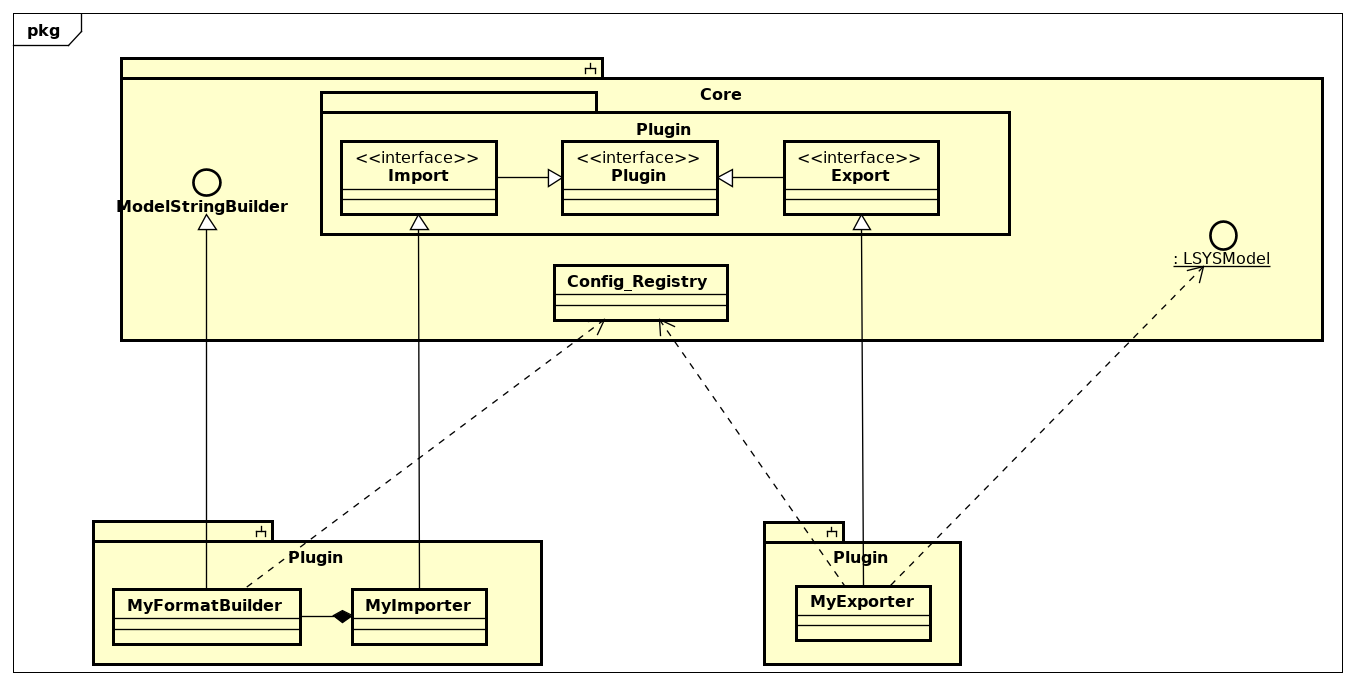
\includegraphics[width=\textwidth]{PluginInterface}
	\caption{Plugin Interface}
	\label{fig:plugint}
\end{figure}

Four plugins were implemented in the course of this thesis
\begin{itemize}
	\item \gls{lsys} Import
	\item Export to \gls{svg}
	\item Export to PDF
	\item Export to STDOUT
\end{itemize}

With the exception of the STDOUT exporter, which is trivial and will not be discussed here, we discuss the plugin implementations.

\subsection{\gls{lsys} Input}
\label{sec:lsys}

This plugin implements the iteration of a given \gls{lsys} description as shown in table \ref{desc:lsysit} to generate a model string.
As this task is critical to overall application performance, an efficient algorithm for iteration has to be selected. 

We decided to use the \class{stringsubst} algorithm from the \term{fxtlib}\furl{https://jjj.de/fxt/fxtpage.html} as recommended by Prof. Arndt.

\subsection{\gls{svg} Output}
\label{sec:svg}
As stated in section \ref{sec:bbcalc}, \gls{svg} and PDF output both precalculate the bounding box and apply the resulting transformation to \class{QPainter} before issuing drawing calls.

A \gls{svg} - unlike PDF - does not have a fixed maximum drawing or paper size, thus the painter need only be translated to avoid drawing at negative coordinates.

Figure \ref{fig:plugsvg} shows a \gls{svg} rendering of the \textsc{R5-Dragon} converted to pdf for inclusing using the \LaTeX\ package \cmd{svg}. The \textsc{R5-Dragon} is a \gls{pfc} on the square grid, whose \gls{lsys} is given in \citet{Arndt2016}[p.23] and was created using 
\begin{lstlisting}[language=bash]
$ ./pfcrender lsys --clear   --it 5 --rules "F F F+F+F-F-F_ + + - - _ _ ~ ~" --sw 2 --sl 10 --rd 0.33 --batch svg --a 90
\end{lstlisting}

\begin{figure}
	\includesvg[width=\textwidth]{SVGexport.svg}
	\caption{\gls{svg} Output of a 5th iterate \textsc{R5-Dragon}}
	\label{fig:plugsvg}
\end{figure}
\subsection{PDF Output}
\label{sec:pdf}
PDF Output is implemented to print to a DIN A4 landscape page and scale to fill it while keeping the aspect ratio of the original curve.
In subsequent releases, configuration of the output parameters will be implemented as \gls{cli} and \gls{gui} configuration options.

Figure \ref{fig:plugpdf} shows a pdf rendering of \textsc{Gosper's Flowsnake} obtained by running
\begin{lstlisting}[language=bash]
$ ./pfcrender lsys  --rules "L_L L L+R++R-L--LL-R+ R -L+RR++R+L--L-R + + - - _ _ ~ ~" --sw 2 --sl 10  --it 4 --rd 0.5 --ia -60 --a 60 pdf --batch
\end{lstlisting}

\begin{figure}
	\includegraphics[width=\textwidth]{PDFexport}
	\caption{PDF Output of \term{Gosper's flowsnake}}
	\label{fig:plugpdf}
\end{figure}
